\section{Reinforcement Learning}\label{rl}
According to Sutton and Barto's seminal text, reinforcement learning (RL) is a branch of machine learning, based on trial-and-error, that is concerned with sequential decision making \cite{Sutton2018}. An RL agent exists in an environment. Within the environment it can act, and it can make observations of it's state and receive rewards. These two discrete steps, action and observation, are repeated indefinitely with the agent's goal being to make decisions so as to maximise its long term reward --- this scenario is represented diagramatically in Figure \ref{fig:209_reinforcement_learning_problem}.

\begin{figure}[h]
	\centering
	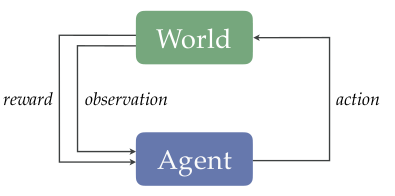
\includegraphics[scale=0.5]{209_reinforcement_learning_problem}
	\caption{text}
	\label{fig:209_reinforcement_learning_problem}
\end{figure}

One of the most common ways to represent the RL problem is to model the environment as a set of discrete probabilistic transitions between states, for a set of possible actions that can be selected by the agent. A state transition presents the agent with a reward signal that informs the agent whether an action taken was good or bad. This environmental architecture is referred to as a Markov Decision Process (MDP). It is the agent's objective to maximise the reward it will receive in the future. An agent can achieve this by learning an optimal policy which maps environment states to actions. Learning such a policy is key idea in RL, and the agent achieves this by experimentation.

%------------------------ SS: MDP

\subsection{Markov Decision Process}
Bellman's pioneering work on the Markov Decision Process (MPD) provided the necessary architecture to develop RL algorithms \cite{Bellm1957}. His work considered an agent that exists in some environment described by a set of discrete states $S$. At any discrete point in time the agent can take an action from the set of possible actions $A$. When the agent takes an action in a given state, the agent receives some reward that is assigned according to a reward function $R: S \times A \times S \to [R_{min}, R_{max}]$. Fundamental to Bellman's MDPs were the state transition dynamics which were defined by probabilities: if an agent is in a given state, $s \in S$, and takes action, $a \in A$, this will transition the agent to a new state, $s' \in S$, and yield reward, $r \in R$, with some given probability. This set of probabilities are assigned by a state transition function $P: S \times A \to S$. Generally, the a single reward is bound to a state transition so function $P$ can be thought to assign a state and reward. The function $P$, and it's simpler notation $p$, is typically written as
\begin{equation}
	P(S_{t+1} = s', \ R_{t+1} = r \ | \ S_t = s, \ A_t = a) = p(s', r \ | \ s, a). \label{eq:202}
\end{equation}

The set of parameters outlined above, and expression \ref{eq:202}, make up a framework referred to as an MDP.

\begin{figure}[h]
\centering
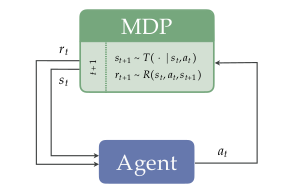
\includegraphics[scale=0.5]{210_reinforcement_learning_problem_mdp}
\caption{text}
\label{fig:210_reinforcement_learning_problem_mdp}
\end{figure}

%------------------------ SS: Returns and Policy

\subsection{Returns, Episodes, and Policy} \label{rep}
In addition to  developing the MDP framework, Bellman was also responsible for key developments in a field of research called dynamic programming (DP) \cite{Bellm1954}. Assuming that the agent has complete knowledge of the state transition probabilities of an environment, DP algorithms can be used to determine analytical solutions for the problem of how an agent should behave to maximise it's cumulative reward \cite{Bellm1954, Howard1960}. This idea was originally thought to be distinct from RL. The main difference is that DP provides the agent with complete knowledge of it's environment, whereas RL agents have no knowledge of environment dynamics and must learn them as well as how to maximise their cumulative reward \cite{Sutton2018}. Many researchers made links between DP and RL \cite{Bellm1959, Witten1977, Werbos1987}, but it wasn't until 1989 that Watkins presented the first formal treatment of RL in an MDP framework. Watkin's work showed that DP algorithms could be modified for use with RL problems \cite{Watkins1989}. Central ideas used in DP algorithms include episodes, returns, and policies \cite{Sutton2018}.

The duration of time that an agent will spend taking actions and transitioning states before encountering a terminal state is defined as an episode. It is the agent's goal to take actions such that it maximises the sum of all the rewards as it concludes an episode. The cumulative sum of rewards is called the return. Consider an agent taking an action at each discrete time step, $t$, and receiving reward, $r_t$, after each action. If there are $N$ discrete time steps before the agent reaches a terminal state, Bellman defines the return as
\begin{equation}
	G_t = \sum_{k = 0}^{N-1} r_{t + k}. \label{eq:203}
\end{equation}

Rewards received in the future are often perceived as less valuable than rewards received in the present. To account for this Bellman used a discount factor applied to each reward in the sequence. Letting $\gamma \in [0,1]$ then \ref{eq:203} becomes
\begin{equation}
	G_t = \sum_{k = 0}^{N-1}\gamma\mystrut^k r_{t+k}. \label{eq:204}
\end{equation}

Finally, in order for the agent to take actions it must have a belief of what action it should take, given it's current state. This belief is called a policy and denoted as $\pi$ \cite{Sutton2018}. Sutton and Barto define a  policy as the mapping of states to actions i.e. a rule that determines what actions the agent should take for a given state. A policy can be deterministic, and depend only on the state, $\pi(s)$, or stochastic, $\pi(a|s)$, such that it defines a probability distribution over the actions, for a given state. An optimal policy, denoted $\pi*$, is a policy which will maximise the return an agent receives over an episode.

%------------------------ SS: Value Function and Bellman

\subsection{Value Function and the Bellman Equations}
The basic principal of dynamic programming is to assign a value to each state that informs an agent how useful a state is to achieving a high cumulative reward. Watkins refers to the creation of systems to assign values to states as the credit assignment problem \cite{Watkins1989}. Bellman's approach to solving credit assignment was to develop mathematical functions to assign values to states \cite{Bellm1954}. Bellman's \textit{value function}, $V_{\pi}(s)$ , is defined as the expected sum of the discounted return, $G_t$, that the agent will receive while following policy $\pi$ from a particular state $s$. Mathematically, this is expressed as
\begin{equation}
	V_{\pi}(s) = \mathbb{E}_{\pi} \big( G_t \ | \ s_t = s \big) = \mathbb{E}_{\pi} \bigg( \sum_{k = 0}^{\infty} \gamma\mystrut^k r_{t+k} \ | \ s_t = s \bigg). \label{eq:205}
\end{equation}

A slight variation of equation \ref{eq:205} is the \textit{state-action value function}, $Q_{\pi}(s,a)$, which is defined as the expected sum of the discounted return, $G_t$, that the agent will receive if it takes action $a$ in state $s$, and then follows policy $\pi$ thereafter. Mathematically, this is expressed as
\begin{equation}
	Q_{\pi}(s, a) = \mathbb{E}_{\pi} \big( G_t \ | \ s_t = s, \ a_t = a \big) = \mathbb{E}_{\pi} \bigg( \sum_{k = 0}^{\infty} \gamma\mystrut^k r_{t+k} \ | \ s_t = s, \ a_t = a \bigg). \label{eq:206}
\end{equation}

Bellman used the value functions presented in \ref{eq:205} and \ref{eq:206} to formulate recursive expressions which could then be used to solve the DP problem \cite{Bellm1957}. These are known as the \textit{Bellman equations}. It is clear the agent would prefer policy $\pi$ over some other policy $\pi'$ provided the expected return from using policy $\pi$ is greater than the expected return from using policy $\pi'$ for all $s \in S$. Since the value function is defined by the expected return, Bellman expressed this idea in value function terms i.e. if policy $\pi$ is preferred to $\pi'$ then $V_{\pi}(s) \geq V_{\pi'}(s)$ for all $s \in S$. Thus, the optimal value function, $V^*(s)$, can be defined as
\begin{equation}
	V^*(s) = \max_{\pi} V_{\pi}(s), \ \forall \ s \in S.
\end{equation}

Similarly, the optimal state-action value function, $Q^*(s,a)$, can be defined as,
\begin{equation}
	Q^*(s,a) = \max_{\pi} Q_{\pi}(s,a), \ \forall \ s \in S, \ a \in A.
\end{equation}

Letting $A(s)$ be the set of actions available in state $s$, if the agent is operating under the optimal policy $\pi^*$ then it is true that
\begin{equation}
	V^*(s) = \max_{a \in A(s)} Q_{\pi*}(s,a). \label{eq:207}
\end{equation}

Using the notation shown in equation \ref{eq:202}, equation \ref{eq:207} can be rewritten using equation \ref{eq:206}
\begin{equation}
	V^*(s) = \max_{a} \sum_{s',r} p(s', r \ | \ s, a)[r + \gamma V^*(s')]. \label{eq:208}
\end{equation}  

Equation \ref{eq:208} is referred to as the Bellman optimality equation for $V^*(s)$. The Bellman optimality equation for $Q^*(s,a)$ is
\begin{equation}
	Q^*(s,a) = \sum_{s'} p(s', r \ | \ s, a)[r + \gamma \max_{a'} Q^*(s',a')].
\end{equation}

If the transition probabilities and rewards are known to the agent then the Bellman opitmality equations can be solved iteratively, which is known as dynamic programming \cite{Bellm1957}. Algorithms which assume probabilities are collectively referred to as \textit{model-based} algorithms. Most RL problems assume state transition probabilities are unknown. The collection of algorithms that provide solutions to these problems are called \textit{model-free} algorithms. Monte Carlo, temporal difference, and policy search are the most common types of model-free algorithms used.

\subsection{Value Function Based Methods}
what are these? why are they used? what is good about them? what are the types?

\begin{figure}[h]
	\centering
	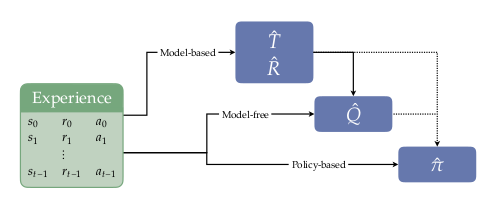
\includegraphics[scale=0.5]{211_families_of_RL_algorithms}
	\caption{text}
	\label{fig:211_families_of_RL_algorithms}
\end{figure}

\subsubsection{Monte Carlo Methods}
Sutton and Barto first introduced a version of the Monte Carlo (MC) control algorithm for estimating state-action value functions in 1998 \cite{Sutton2018}. The basic idea is based on an iterative approach that takes a sample of episodic sequences consisting of states, actions, and rewards. Sequences are obtained from the agent interacting with the environment, using some policy $\pi$. This is called the \textit{policy evaluation} step. Once an episode is completed, the state-action value function, $Q_{\pi}(s,a)$, is updated for each discrete state-action pair visited. This second step is called the \textit{policy improvement} step. Figure \ref{fig:210_monte_carlo_methods} illustrates the iterative process.

Greedy policy talk about this guy too
\begin{equation}
	\pi (a | s) = % 
	   \begin{cases}
	   		1 \ \ \text{if} \ \ a = \arg\max_{a'} Q(s,a') \\
	   		0 \ \ \text{if} \ \ a \neq \arg\max_{a'} Q(s,a')
	   \end{cases}
\end{equation}


Need to talk about greedy and epsilon greedy policies and their motivation first.
\begin{equation}
   \pi (a | s) = % 
   \begin{cases}
   		1 - \epsilon \ \ \text{if} \ \ a = \arg\max_{a'} Q(s,a') \\
   		\frac{\epsilon}{|A|-1} \ \ \text{if} \ \ a \neq \arg\max_{a'} Q(s,a')
   \end{cases}
\end{equation}



\begin{figure}[h]
	\centering
	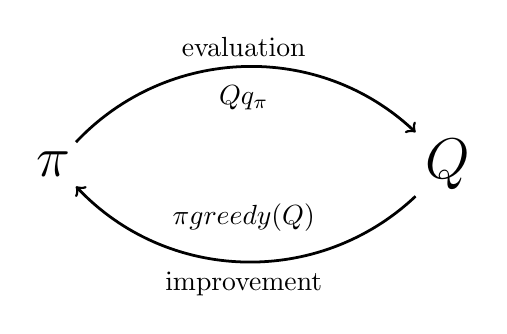
\begin{tikzpicture}
	
	% Create nodes
	\node (A) {\huge$\pi$};
	\node[right of=A, node distance=5cm] (B) {\huge$Q$};
	
	% Create arrow
	\draw[->, line width=1pt] (A) edge[bend left=45] node[below=0.1cm] {$Q \rightsquigarrow q_\pi $} node[above] {evaluation} (B);
	
	% Create arrow
	\draw[->, line width=1pt] (B) edge[bend left=45] node[below] {improvement} node[above=0.25cm] {$\pi \rightsquigarrow greedy(Q)$} (A);
	
\end{tikzpicture}
	\caption{text}
	\label{fig:210_monte_carlo_methods}
\end{figure}

\begin{algorithm}[h]
	\caption{Constant $\alpha$ Monte Carlo Control}
	\label{alg:01_monte_carlo}
	\begin{algorithmic}[1]
		\State{\textbf{Input:} $\mathtt{num\_episodes}$, $\alpha$, $\epsilon_i$}
		\State{\textbf{Output:} $\pi$ ($\approx \pi^*$ if $\mathtt{num\_episodes}$ is large enough)}
		\State{Initialise $Q$ such that $Q(s,a) = 0 \ \text{for all} \ s \in A \ \text{and} \ a \in A$}
		\For{$i \gets 1:\mathtt{num\_episodes}$}
			\State{$\epsilon \gets \epsilon_i$}
			\State{$\pi \gets \epsilon-\text{greedy}Q$}
			\State{Generate and episode $S_0, A_0, R_1,\dots,S_T$ using $\pi$}
			\For{$t \gets 0:(T-1)$}
				\If $(S_t, A_t)$ is a first visit
					$Q(S_t, A_t) \gets Q(S_t, A_t) + \alpha(G_t - Q(S_t, A_t))$
				\EndIf
			\EndFor
		\EndFor
		\State{\textbf{return} $Q$}
	\end{algorithmic}
\end{algorithm}



\subsubsection{Temporal Difference Methods}
Talk about the fact that Monte Carlo methods collect an entire episode prior to making an update - temporal difference methods use an idea of bootstrapping to update the Q after each time step. This has low bias but high variance (check this idea)?


Watkins is credited with the most influential integration of RL with MDPs, and DP. His work on an RL algorithm called Q-learning highlighted the importance of another type of value function called the action-value function. The action-value function is defined as the expected sum of rewards that the agent will receive while taking action $a$ in state $s$ and, thereafter, following policy $\pi$.

\begin{equation}
	Q(s,a) := Q(s,a) + \alpha[r + \max_{a'}Q(s',a') - Q(s,a)]
\end{equation}

\begin{algorithm}[h]
	\caption{Q-learning}
	\label{alg:02_q_learning}
	\begin{algorithmic}[1]
		\State{\textbf{Input:}}
		\State{\textbf{Output:}}
		\State{Initialise $Q(s,a)$ randomly}
		\Repeat
			\State{Observe initial state $s_1$}
			\For{$t \gets 1:T$} 
				\State{Select an action $a$ using policy derived from $Q$ (e.g. $\epsilon$-greedy)}
				\State{Carry out action $a$}
				\State{Observe reward $r$ and new state $s'$}
				\State Update {$Q(s,a) \gets Q(s,a) + \alpha[r + \max_{a'} \gamma Q(s',a') - Q(s,a)]$}
			\EndFor
		\Until{Terminated}
	\end{algorithmic}
\end{algorithm}


\subsection{Policy Search Methods}

\subsection{Actor Critic Methods}